\documentclass{article}           %% ceci est un commentaire (apres le caractere %)
%%\usepackage[latin1]{inputenc}     %% adapte le style article aux conventions francophones
%%\usepackage[T1]{fontenc}          %% permet d'utiliser les caractères accentués
\usepackage[utf8]{inputenc}
\usepackage[T1]{fontenc}
\usepackage[dvips]{graphicx}      %% permet d'importer des graphiques au format .EPS (postscript)
\usepackage{fancybox}		   %% package utiliser pour avoir un encadré 3D des images
\usepackage{makeidx} 

\usepackage{lmodern} %Ty 
            %% permet de générer un index automatiquement
%\usepackage{subfig} %%Teilabbildungen in einer Abbildung
%\usepackage{pst-all} %%PSTricks - nicht verwendbar mit pdfLaTeX

%% Beachten Sie:
%% Die Einbindung einer Grafik erfolgt mit \includegraphics{Dateiname}
%% bzw. über den Dialog im Einfügen-Menü.
%% 
%% Im Modus "LaTeX => PDF" können Sie u.a. folgende Grafikformate verwenden:
%%   .jpg  .png  .pdf  .mps
%% 
%% In den Modi "LaTeX => DVI", "LaTeX => PS" und "LaTeX => PS => PDF"
%% können Sie u.a. folgende Grafikformate verwenden:
%%   .eps  .ps  .bmp  .pict  .pntg


%% Packages für Formeln %%%%%%%%%%%%%%%%%%%%%%%%%%%%%%%%%%%%%
\usepackage{amsmath}
\usepackage{amsthm}
\usepackage{amsfonts}

\usepackage[french]{babel}
\usepackage{fullpage}
\usepackage{eso-pic}
\usepackage{textcomp}
\begin{center}

\usepackage{multirow}					
\title{ les m\'ethodes de gestion de projet agile}     %% \title est une macro, entre { } figure son premier argument
\author{Laby Damaro CAMARA}        %% idem
\makeindex		    %% macro qui permet de générer l'index
\bibliographystyle{prsty}	  %% le style utilisé pour créer la bibliographie
\begin{document}                  %% signale le début du document
\maketitle                        %% produire à cet endroit le titre de l'article à partir des informations fournies ci-dessus (title,author)
\title{La m\'ethode Scrum}
\newpage
\tableofcontents                  %% produire à cet endroit la table des matièree					           
\section{Le choix de la m\'ethode de gestion de projet}
Le choix de la m\'ethode de d\'eveloppement s’est port\'e vers la m\'ethode SCRUM.
SCRUM est la m\'ethode Agile la plus utilis\'ee parmi les autres m\'ethodes Agile. Et de fait, la
plus \'eprouv\'ee.

D’autre part, SCRUM est un processus it\'eratif et incr\'emental, repr\'esente un framework
de d\'eveloppement logiciel agile pour la gestion du d\'eveloppement des produits.
Il d\'efinit « une approche souple, strat\'egie de d\'eveloppement de produits holistique et permet
aux \'equipes de d\'eveloppement de s'organiser comme une unit\'e pour atteindre un objectif
commun ».

L’une des particularit\'es de SCRUM est que pendant le d\'eveloppement de produits, les clients
peuvent changer d'avis sur ce qu'ils veulent et ont besoin (souvent appel\'e la volatilit\'e des
exigences).

\section{Principe de SCRUM}
SCRUM est une m\'ethode agile d\'edi\'ee à la gestion de projet. Cette m\'ethode de gestion a pour
objectif d’am\'eliorer la productivit\'e de son \'equipe.

La m\'ethode SCRUM implique que le projet progresse à travers la mise en place de s\'eries de «
sprints ». A chaque lancement d’un sprint, une r\'eunion de planification est organis\'ee afin que
chaque membre de l’\'equipe puisse s’engager sur le nombre de tâches qu’il pourra ex\'ecuter,
ainsi que sur la cr\'eation du « sprint blacklog », qui est la liste globale des tâches à r\'ealiser lors
du sprint.

Chaque jour du sprint, tous les membres de l’\'equipe (ainsi que le responsable produit et le
SCRUM Master) doivent assister à la r\'eunion SCRUM quotidienne. Cette dernière ne doit pas
durer plus de 15 minutes, et permet aux membres de l’\'equipe de partager aux autres ce qu’ils 
P a g e 32 | 92
ont fait la veille, ce sur quoi ils travaillent le jour même, ainsi que l’identification de tout
problème pouvant entraver le bon d\'eroulement du sprint. Cette r\'eunion permet ainsi de
synchroniser tous les membres de l’\'equipe.
La fin d’un sprint est marqu\'ee par une session de d\'ebriefing permettant de pr\'esenter le travail
achev\'e au responsable produit, et de partager des informations pouvant influer sur le sprint
suivant.
Voilà un sch\'ema qui repr\'esente le processus de la m\'ethodologie SCRUM, avec un d\'etail de
chaque \'etape :
\begin{figure}[!h]
	\begin{flushleft}
		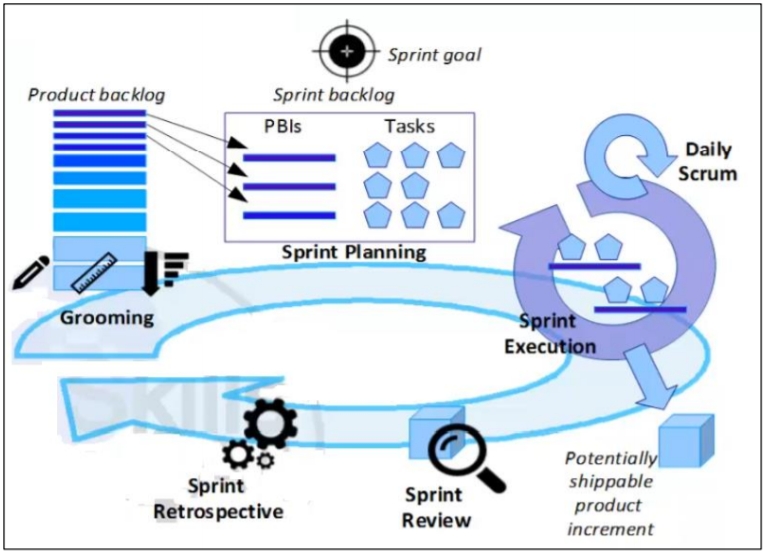
\includegraphics[width=450pt, height=250pt]{images/scrum.png}
	\end{flushleft}
	\caption{ D$é$marche du projet}
	\label{ Démarche du projet}
\end{figure}

\subsection{Product backlog}
Les utilisateurs constituent un produit de backlog, qui va être composé de toutes les demandes
de fonctionnalités priorisées. C’est pour cela que dans le produit backlog, on a le dépile par le
haut, et le haut du produit backlog représente les fonctionnalités les plus demandées et les plus
urgentes, qu’il va falloir réaliser en premier. 

\subsection{Sprint planning}
Comme l’indique le schéma, on va sélectionner les PBI « les produits de backlog items » qui
sont les plus demandés par l’utilisateur, c’est-à-dire qui sont en haut de la pile. Puis dans le
sprint planning on va décomposer les PBIs en taches auxquelles on va donner une durée en
heures.
\subsection{Sprint execution}
Une fois on a fait ce spring palnning c’est-à-dire qu’on a déterminé l’ensemble des taches qui
vont être réalisées pendant cette itération ce qu’on appelle un sprint. Eh bien là, on va exécuter
l’itération, dans sprint execution, et c’est là où on a une équipe de projet, une équipe de
développement qui vont réaliser les incréments de fonctionnalités.

\subsection{Daily scrum}
Tous les jours on a un petit événement qui s’appelle le daily scrum pendant lequel on passe en
revue ce qui a été développé la veille, ce qui sera développé demain et comment on va s’y
prendre.

Cet événement très court qui prend peu de temps « point rapide sur ce qui s’est déroulé la veille,
sur ce qui doit se dérouler aujourd’hui et puis suivant le travail ».


\subsection{Potentially shippable product increment}
Une fois qu’on a fait l’ensemble des itérations, normalement on devrait avoir vingt itérations à
peu près égales, maintenant on va avoir probablement un ou plusieurs incréments de
fonctionnalités qui sont potentiellement intégrables dans le produit.
C’est pour cela qu’on parle en anglais de Potentially shippable product increment, c’est-àdire à la fin de mon itération je ne vais pas forcément livrer quelque chose, en tout cas, j’ai
quelque chose qui devrait pouvoir être mis en production, peut-être pas la fin de cette itération,
peut-être la fin d’une autre itération, mais c’est quelque chose de tangible.
Donc on va montrer tout cela aux utilisateurs pour avoir le retour hi-média, et d’ailleurs une
fois qu’on a montré aux utilisateurs ce qui convient de développer, ils vont pouvoir donner
l’accord, faire des modifications ou ajouter de nouveaux PBIs.

\subsection{Sprint Review}
L’évènement suivant c’est sprint review, dans lequel on passe en revue ce qui a été réalisé
pendant l’itération avec l’utilisateur et puis le passer à ce moment-là avec ce qui «est demandé
par les utilisateurs, de ce qu’il va falloir encore ajouter au produit backlog, ou supprimer. C’est
à ce moment-là qu’on fait la revue de ce que le sprint a délivré

\subsection{Sprint retrospective}
C’est la dernière étape dans cette méthodologie, est là on passe en revue les éléments de la
méthodologie Scrum dans l’entreprise « ce qui a fonctionné ou ce qui n’a pas fonctionné, en
fait, c’est une revue de la méthodologie ».

\subsection{Les Rôles de Scrum}
Scrum définit seulement 3 rôles :
\item[Le Product Owner :] qui porte la vision du produit à réaliser et travaille en interaction
avec l’équipe de développement. Il s’agit généralement d’un expert du domaine métier
du projet.
\item[L’Equipe de Développement:] qui est chargée de transformer les besoins exprimés par le
Product Owner en fonctionnalités utilisables. Elle est pluridisciplinaire et peut donc
encapsuler d’autres rôles tels que développeur, architecte logiciel, DBA, analyste
fonctionnel, graphiste/ergonome, ingénieur système.
\item[Le Scrum Master: ] qui doit maîtriser SCRUM et s’assurer que ce dernier est correctement
appliqué. Il a donc un rôle de coach à la fois auprès du Product Owner et auprès de
l’équipe de développement. Il doit donc faire preuve de pédagogie. Il est également
chargé de s’assurer que l’équipe de développement est pleinement productive. 


\end{document} 
